\begin{figure}
\centering
\begin{tikzpicture}
  % variables
  \def\n{7}; \def\nodespan{0.7}; \def\xarrowlen{1}; 
  \def\layerlen{4}; \def\arrowspacing{1};

  \coordinate (repere) at (-1.2*\arrowspacing, -3*\nodespan);
  % Draw the x-axis
  
  \draw[ultra thick, -Latex] (repere) --  ++ (0, \xarrowlen) node[right] {$x_2$};
  \draw[ultra thick, -Latex] (repere) -- ++ (\xarrowlen, 0) node[below right] {$x_1$};
  % geometry drawing
  \fill[gris2!50!white] (0, -1*\nodespan) 
        rectangle ++ (\layerlen, 2*\nodespan);
  % Domains legends 
  \draw[thick, black] (0, -1*\nodespan) node[above right] {$\Gamma^{(n)}$}
        -- (\layerlen, -1*\nodespan) ;
  \draw[thick, black] (0, 1*\nodespan) node[above right] {$\Gamma^{(n+1)}$}
        -- (\layerlen, 1*\nodespan) ;
  \draw[thick, black] (0, -1*\nodespan) 
        -- (\layerlen, -1*\nodespan) node[midway, below] {$\vdots$};
  \draw[thick, black] (0, 1*\nodespan) 
        -- (\layerlen, 1*\nodespan) node[midway, above] {$\vdots$};
  % Draw Chebyshev nodes
  \foreach \i in {0,...,\n} {
    \pgfmathsetmacro\x{\nodespan*cos((\i+0.5)*180/(\n+1))}
    \draw[black, fill=black] (3/4*\layerlen, \x) circle (0.8pt);
    };
    % Draw other elements
    \draw[Latex-] (3/4*\layerlen, .38) 
    to[bend left] ++ (-.4, .9) node[above] {node $\xi_i $};
    \draw[-Latex] (\layerlen*0.3, -0.1*\nodespan) 
    -- ++ (1, 0) node[midway, above] {$ k_1$};
    \draw[Latex-Latex] (0.3-\arrowspacing, -1*\nodespan) 
    -- ++ (0, 2*\nodespan) node[midway, left] {$h^{(n)}$};
    \draw[Circle-] (\layerlen-0.3, 0) 
    -- ++ (\arrowspacing, 0) node[right] {$\Omega^{(n)}$};
%     % Add 3D view of the geometry
%     \node[left] at (-2.3, 0) {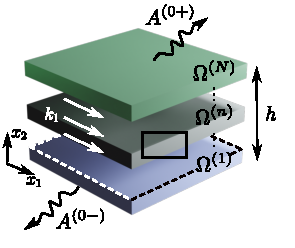
\includegraphics[scale=1.5]{multilayerdiagram_3Dview.pdf}};
    % subfigure nodes
    \node at (-5.7, -.55) {b)};
    \node at (-8.5, 2.5) {a)};    
    \node at (-1.5, 2.5) {b)};
\end{tikzpicture}
    \caption{a) Sketch of the geometry of the multilayer system and b) zoom on the $n$-th layer.}
    \label{fig:schema_multilayer}
\end{figure}